\chapter{Questions}

\section{Probability}

1. Let P and Q be two probability distributions, where Q is parametric. Which of the following sentences about the Kullback-Leiber divergence is true?

\begin{enumerate}[label=\roman*]
    \item KL divergence is a distance between two probability distributions.
    \item KL divergence is a measure of the dissimilarity between two probability distributions.
    \item KL divergence is the same as Cross-Entropy
    \item Minimizing the Cross-Entropy of P with respect to Q is equivalent to minimizing the KL divergence between P and Q.
    \item Minimizing the Mean Squared Error of P with respect to Q is equivalent to minimizing the KL divergence between P and Q.
\end{enumerate}

\noindent 2. Let $ p_{model} (x, \theta)$ be a parametric family of probability distribution that maps the samples giving as a result an estimation of the true distribution $p_{data} (x)$. Which of the following questions are WRONG?

\begin{enumerate}[label=\roman*]
    \item Maximum Likelihood estimation is a special case of Maximum A Posteriori estimation.
    \item Maximum Likelihood assumes a uniform prior of the hypothesis.
    \item Maximum Likelihood approaches make predictions using a full probability distribution over $\theta$.
    \item Minimizing $D_{KL} (p_{data} || p_{model})$ is the same as minimizing the Cross-Entropy between the two distributions.
    \item None.
\end{enumerate}

\section{Learning with Gradient}

1. Which of the following sentences about the condition number is WRONG?

\begin{enumerate}[label=\roman*]
    \item Condition number gives information about the curvature in the different dimensions.
    \item The condition number is the ratio between the maximum and minimum nonzero eigenvalues of the Jacobian matrix.
    \item The speed of convergence of the Gradient Descent is dependent on the Condition Number.
    \item Computing the Condition Number is computationally demanding.
    \item None. 
\end{enumerate}

\noindent 2. What is the condition number of a Hessian matrix? In which context is used in optimizing a Deep Learning model?

\newpage
\section{Neural Networks}

1. Which one of the following is an advantage of using Deep Neural Networks over linear models?

\begin{enumerate}[label=\roman*]
    \item A Deep Neural Network has the same expressive power of linear models.
    \item A Neural Network always performs better than linear models.
    \item A Deep Neural Network has better generalization than a linear model.
    \item The functions we want to learn are always a composition of simpler functions, so Deep Neural Networks are always more suited for learning problems.
    \item None of the above
\end{enumerate}

\noindent 2. For which label distribution and which loss is reasonable to adopt the softmax activation function for the output layer?

\begin{enumerate}[label=\roman*]
    \item Gaussian distribution / Mean Squared Error
    \item Gaussian distribution / Cross-Entropy
    \item Multinoulli distribution / Cross-Entropy
    \item Multinoulli distribution / Mean Squared Error
\end{enumerate}


\noindent 3. For which label distribution and which loss is reasonable to adopt the sigmoid activation function for the output layer, according to the max likelihood principle?

\begin{enumerate}[label=\roman*]
    \item Gaussian distribution / Mean Squared Error
    \item Gaussian distribution / Cross-Entropy
    \item Multinoulli distribution / Cross-Entropy
    \item Bernoulli distribution / Cross-Entropy
    \item None of the above
\end{enumerate}

\noindent 4. For which label distribution and with which loss is reasonable to adopt the linear activation function for the output layer?

\begin{enumerate}[label=\roman*]
    \item Gaussian distribution / Mean Squared Error
    \item Gaussian distribution / Cross-Entropy
    \item Multinoulli distribution / Cross-Entropy
    \item Multinoulli distribution / Mean Squared Error
\end{enumerate}

\newpage
\noindent 5. Which of the following statements about the Universal Approximation Theorem for Neural Networks is true? 

\begin{enumerate}[label=\roman*]
    \item A Neural Network with at least two hidden layers and a squashing activation function can approximate any continuous function.
    \item A Neural Network with at least one hidden layer and a squashing activation function can approximate arbitrarily well any continuous function with any number of hidden neurons.
    \item A Neural Network with one hidden layer and a squashing activation function can approximate arbitrarily well any continuous function given enough hidden neurons.
    \item The minimum number of neurons required for a Neural Network with one hidden layer and a squashing activation function to approximate up to a given extent a continuous function is linear in the input dimension.
    \item The number of hidden neurons required for a Neural Network with many hidden layers and a squashing activation function to approximate up to a given extent a continuous function is linear in the depth of the network.
\end{enumerate}

\noindent 6. Consider a 3-layers Neural Network defined as follows:

$$ sign (W'''(W''(W'x + b') + b'') + b''')$$

which of the following is true:

\begin{enumerate}[label=\roman*]
    \item The hypothesis space of this model is the sum of the perceptron.
    \item This model can solve the XOR problem.
    \item Adding one more linear hidden layer will increase the expressiveness of the model.
    \item If $W'''$ has more parameters than $W''$ that has more parameters than $W'$, the network is universal approximately. 
    \item None of the above.
\end{enumerate}

\noindent 7. Which of the following statements about the approximation capabilities of Neural Networks is true? 

\begin{enumerate}[label=\roman*]
    \item A Neural Network with at least one hidden layer and a squashing activation function can approximate arbitrarily well any continuous function with any number of hidden neurons.
    \item The minimum number of hidden neurons required for a Neural Network with two hidden layers and a squashing activation function to approximate up to a given extent a continuous function is linear in the input dimension.
    \item The number of hidden neurons required for a Deep Neural Network with many hidden layers and a squashing activation function to approximate up to a given extent a continuous function cannot be exponential in the input size.
    \item A Neural Network with four hidden layers and a squashing activation function can approximate arbitrarily well any continuous function given enough hidden neurons. 
    \item None of the above.
\end{enumerate}


\noindent 8. Can the following equation

$$ sign (W'''(W''(W'x + b') + b'') + b''')$$

solve the XOR problem? Why or why not? If not modify it as little as possible so it can.

\noindent 9. Why is it convenient to have more than one hidden layer in a Neural Network? In other words, what is the advantage of a multi-layer Neural Network over a single-hidden-layer Neural Network?

\noindent 10. How can the maximum likelihood principle be exploited to choose the most suitable activation function for the neurons in a NN?

\noindent 11. Explain which activation function for the output layer, and loss function should we choose when facing a regression problem, according to the maximum likelihood principle. Motivate your answer, explaining which assumptions we are making and how we are modelling the output of the NN from a probabilistic perspective.

\section{Backpropagation}


1. What is the difference between backpropagation and SGD?

\noindent 2. Given a Neural Network described by the following equations:

$$ h^{(1)} = W^{(1)}x + b^{(1)}  ~~~~~ a^{(1)} = ReLU(h^{(1)}) ~~~~~ h^{(2)} = (w^{(2)})^{T} a^{(1)} + b^{(2)} ~~~~~ y = \sigma(h^{(2)}) ~~~~~ J = \frac{1}{2} \left ( t - y \right)^{2} $$

\noindent with $ x = \begin{pmatrix} 1 \\ 0.5 \end{pmatrix} $, $ W^{(1)} = \begin{pmatrix} 0.75 & 0.5 \\ -1 & 1  \end{pmatrix} $, $ b^{(1)} = \begin{pmatrix} 0 \\ 0 \end{pmatrix} $, $w^{(2)} = \begin{pmatrix} 1 \\ 1 \end{pmatrix}$, $b^{(2)} = -1$ and $ t=1 $ compute the value of $ \frac{\partial J}{\partial W_{1, 1}^{(1)}} $ (Hint $\sigma (0) = 0.5$).



\noindent 3. Given a Neural Network described by the following equations:

$$ h^{(1)} = W^{(1)}x + b^{(1)}  ~~~~~ a^{(1)} = ReLU(h^{(1)}) ~~~~~ h^{(2)} = (w^{(2)})^{T} a^{(1)} + b^{(2)} ~~~~~ y = \sigma(h^{(2)}) ~~~~~ J = \frac{1}{2} \left ( t - y \right)^{2} $$

\noindent with $ x = \begin{pmatrix} 0.5 \\ 1 \end{pmatrix} $, $ W^{(1)} = \begin{pmatrix} 0.5 & 0.75 \\ 1 & -1  \end{pmatrix} $, $ b^{(1)} = \begin{pmatrix} 0 \\ 0 \end{pmatrix} $, $w^{(2)} = \begin{pmatrix} 1 \\ 2 \end{pmatrix}$, $b^{(2)} = -1$ and $ t=1 $ compute the values of $ \frac{\partial J}{\partial W^{(1)}} $ and $ \frac{\partial J}{\partial W^{(2)}} $ (Hint $\sigma (0) = 0.5$).


\noindent 4. Given a Neural Network described by the following equations:

$$ h^{(1)} = W^{(1)}x + b^{(1)}  ~~~~~ a^{(1)} = ReLU(h^{(1)}) ~~~~~ h^{(2)} = (w^{(2)})^{T} a^{(1)} + b^{(2)} ~~~~~ y = \sigma(h^{(2)}) ~~~~~ J = \frac{1}{2} \left ( t - y \right)^{2} $$

\noindent with $ x = \begin{pmatrix} 0.5 \\ 1 \end{pmatrix} $, $ W^{(1)} = \begin{pmatrix} 0 & 0 \\ 1 & -1 \\ 1 & 1.5 \end{pmatrix} $, $ b^{(1)} = \begin{pmatrix} -1 \\ 0 \\ 0 \end{pmatrix} $, $w^{(2)} = \begin{pmatrix} 0 \\ 3 \\ 1 \end{pmatrix}$, $b^{(2)} = -2$ and $ t=1 $ compute the values of $ \frac{\partial J}{\partial W^{(1)}} $ and $ \frac{\partial J}{\partial W^{(2)}} $ (Hint $\sigma (0) = 0.5$).

\noindent 5. Given a Neural Network described by the following equations:

$$ h^{(1)} = W^{(1)}x + b^{(1)}  ~~~~~ a^{(1)} = \sigma(h^{(1)}) ~~~~~ h^{(2)} = (w^{(2)})^{T} a^{(1)} + b^{(2)} ~~~~~ y = \sigma(h^{(2)}) ~~~~~ J = \frac{1}{2} \left ( t - y \right)^{2} $$

\noindent with $ x = \begin{pmatrix} 1 \\ 0.5 \end{pmatrix} $, $ W^{(1)} = \begin{pmatrix} -1 & 1 \\ 0 & 0 \end{pmatrix} $, $ b^{(1)} = \begin{pmatrix} 0.5 \\ 0 \end{pmatrix} $, $w^{(2)} = \begin{pmatrix} 2 \\ -2 \end{pmatrix}$, $b^{(2)} = 0$ and $ t=1 $ compute the values of $ \frac{\partial J}{\partial W^{(1)}} $ and $ \frac{\partial J}{\partial b^{(1)}} $ (Hint $\sigma (0) = 0.5$).

\newpage
\section{Regularization}

1. Which of the following sentences about regularization are true?

\begin{enumerate}[label=\roman*]
    \item Parameter norm penalties are useless when there is dropout because it is a stronger regularizer.
    \item Dropout is useless when parameter norm penalties are used because it is a stronger regularizer.
    \item With parameter norm penalties, the higher we weight the norm, the more the model is regularized.
    \item Weight decay is the same as L1 regularization.
    \item Weight decay is the same as L2 regularization.
\end{enumerate}

\noindent 2. Multi-task learning can improve the predictive performance over single task learning.

\begin{enumerate}[label=\roman*]
    \item Because there are more training data to train on.
    \item Because the network is more complex and thus more expressive.
    \item Only if the considered tasks are somehow related.
    \item Only if there are many tasks to use (usually at least 3).
\end{enumerate}

\noindent 3. Which one of the following sentences about regularization are true?

\begin{enumerate}[label=\roman*]
    \item Regularization reduces the training error.
    \item Regularization reduces the generalization error.
    \item Regularization increases the inductive bias of the model.
    \item Regularization increases the variance of the model.
\end{enumerate}

\noindent 4. Explain what is dropout and how it can be implemented in both training and evaluation and why is that. Motivate your answer. Moreover, explain why does it act as a regularization technique.

\section{Optimisation}

1. Which of the following statements about optimisation of a Deep Neural Networks are true?

\begin{enumerate}[label=\roman*]
    \item In the optimisation of Deep Neural Networks, the weights corresponding to low training error are the ones that generalise better.
    \item Minimizing the true error would be more prone to overfitting than minimizing the empirical error.
    \item We don't necessarily need a differentiable loss function to perform Gradient Descent.
    \item Gradient Descent many times converges to the global minima of an optimization problem even though is not guaranteed to do so.
    \item None of the above.
\end{enumerate}

\noindent 2. Which of the following sentences about weight initialisation in Neural Networks is True?

\begin{enumerate}[label=\roman*]
    \item The weight initialization is not important in training Deep Neural Networks.
    \item We can only use unsupervised datasets for pre-training. If we want to exploit an external dataset where there is supervision, we should use multi-task learning.
    \item Pre-training acts as learning bias favouring weights that are close to the ones of the pre-trained model.
    \item Even though different weight initialisation may provide different solutions, usually they provide the same results.
    \item None of the above.
\end{enumerate}

\noindent 3. Which one of the following properties about optimizing the weights of Deep Neural Networks are true?

\begin{enumerate}[label=\roman*]
    \item Local minima are probably associated to high cost.
    \item Gradient clipping can alleviate the vanishing gradient problem.
    \item Gradient clipping can alleviate the exploding gradient problem.
    \item Local minima are probably associated to low cost.
    \item Saddle points are probably associated to low cost.
    \item Saddle points are probably associated to high cost.
\end{enumerate}

\noindent 4. Which one of the following sentences about Second-order optimization methods is WRONG?

\begin{enumerate}[label=\roman*]
    \item They consider the Hessian of the function to optimise.
    \item They are computationally slower, than first-order methods.
    \item If used instead of first-order Gradient Descent, the optimisation will converge faster in terms of number of steps needed.
    \item They are not widely used in optimising Neural Networks because they converge to a worse solution compared to first-order methods.
    \item None of the others.
\end{enumerate}

\noindent 5. Why is mini-batch Gradient Descent commonly used for training Deep Neural Networks instead of Gradient Descent or Stochastic Gradient Descent (online)?

\begin{enumerate}[label=\roman*]
    \item Mini-batch Gradient Descent estimates the gradient better than Gradient Descent.
    \item Mini-batch Gradient Descent estimates the gradient better than online Stochastic Gradient Descent.
    \item The gradient in mini-batch Gradient Descent is faster to compute than Gradient Descent.
    \item The gradient in mini-batch Gradient Descent is faster to compute than online Stochastic Gradient Descent.
    \item The gradient in online Stochastic Gradient Descent is too noisy, and in Gradient Descent it may be too slow to complete.

\end{enumerate}


\noindent 6. What are the main problems we face when optimising Deep Neural networks? For each one, explain why it is a problem for optimisation algorithms. Where applicable, explain how it is possible to avoid such problems.

\noindent 7. Explain the main characteristics and differences among: Gradient Descent, mini-batch Stochastic Gradient Descent, Adagrad, RMSprop and Adam.

\noindent 8. Explain why it is not a good idea to initialise all the weights of a Neural Network to zero. Consider both the cases in which the ReLU activation function is used, and the general case.

\noindent 9. What are local minima and saddle points, and why are them a problem for optimising algorithms?


\newpage
\section{Convolutional Neural Networks}

1. Which one of the following sentences about Unshared Convolution are true?

\begin{enumerate}[label=\roman*]
    \item The unshared convolution is slower compared to standard convolution.
    \item The unshared convolution is faster compared to standard convolution.
    \item The unshared convolution maintains the translational equivarence of the computed representation.
    \item The unshared convolution can be combined with Pooling similarly to standard convolution. In this case the property of producing a representation approximately invariant to small translations still holds.
    \item The unshared convolution can be combined with Pooling similarly to standard convolution. In this case the property of producing a representation approximately invariant to small translations is lost.
    \item None of the above.
\end{enumerate}

\noindent 2. For which reasons using Convolutional Neural Network on images gives, in general, better results than using dense layers?

\begin{enumerate}[label=\roman*]
    \item Because it significantly reduces the number of parameters to learn.
    \item Because is faster.
    \item Because of the translation equivariance given by tied weights.
    \item Because of the translation invariance given by tied weights.
\end{enumerate}

\noindent 3. When the input data are images, the learning bias induced by a Convolutional Neural Network layers allows to improve the predictive performance over a dense layer all the times?

\begin{enumerate}[label=\roman*]
    \item Yes
    \item No
\end{enumerate}


\noindent 4. Consider an unshared Convolutional Neural Network layer with just 1 filter of size $3 \times 3$, a stride of 1, input images of size $4 \times 4$ and no padding. How many parameters are we required to train for such a layer?

\noindent 5. Consider a Convolutional Neural Network layer with 10 filters of $ 4 \times 4$ size, a stride of 1 and input images of $ 8 \times 8$. How many parameters are we require to train for such a layer?

\noindent 6. Consider a Convolutional Neural Network layer with 10 filters of $ 4 \times 4$ size, a stride of 2 and input images of $ 8 \times 8$ on a single channel (black and white). How many multiplications are we required to compute the output of such a layer?

\noindent 7. Consider a Convolutional Neural Network layer with 16 filters of $ 3 \times 3$ size, a stride of 1 and input images of $ 10 \times 10$. How many parameters are we require to train for such a layer?

\noindent 8. Consider a Convolutional Neural Network layer with 10 filters of $ 4 \times 4$ size, a stride of 2 and input images of $ 6 \times 6$ on a single channel (black and white). How many multiplications are we required to compute the output of such a layer?

\noindent 9. Consider a Convolutional Neural Network layer with 10 filters of $ 4 \times 4$ size, a stride of 1 and input images of $ 6 \times 6$ on a single channel (black and white). How many multiplications are we required to compute the output of such a layer?

\noindent 10. Consider a Convolutional Neural Network layer with 3 filters of $ 2 \times 2$ size, a stride of 1 and input images of $ 3 \times 3$. How many summations are we required to compute the output of such a layer? (Consider a summation a two element summation).

\noindent 11. Consider a Convolutional Neural Network layer with 10 filters of $ 2 \times 2$ size, a stride of 2 and input color images (3 input channels) of size $ 16 \times 16$. How many parameters are we required to train for such a layer?

\section{Practical Methodology}

1. Which of the following sentences about model selection is true?

\begin{enumerate}
    \item Using Cross-validation in validating a Neural Network is not correct.
    \item The size of validation and test sets have to be always the same.
    \item Considering 20\% of the data as validation set is always the best setting.
    \item Given a fixed size dataset, it is always true that  the larger the test set, the higher the performance.
    \item None of the above.
\end{enumerate}

\noindent 2. Explain how to correctly select the number of hidden layers and the corresponding activation functions in a Deep Neural Network, why it is important to obtain a correct evaluation of the model's predictive performance. and how we can do that. Discuss the various methodologies also considering the impact in terms of computational burden.

\noindent 3. Explain how to correctly estimate the true error in a Deep Neural Network?



\section{Sequence Modeling: Recurrent and Recursive Nets }

\noindent 1. A sequential transduction is stationary if:

\begin{enumerate}[label=\roman*]
    \item It is causal.
    \item The output is a linear function of its inputs.
    \item Has finite memory.
    \item It can be learned by a feedforward Neural Network with a time window of size equal to the memory of the transduction.
    \item None of the above are correct.
\end{enumerate}

\noindent 2. In order for sequential transductions to have a recursive state representation, the following property should hold:

\begin{enumerate}
    \item The corresponding Recurrent Neural Netowrk should not have short-cut connections from the input to the output.
    \item The corresponding Recurrent Neural Network should have for each hidden state a shift-time connection $q^{-1}$ with $i > 0$.
    \item The transduction should have finite memory.
    \item The transduction should be causal.
    \item Any sequential transduction admits a recursive state representation.
\end{enumerate}


\noindent 3. Consider a time series prediction task where, given a time sequence in input up to time $t$, the output should predict the value of the input at time $t+1$. Which architecture cannot be used to perform the task?

\begin{enumerate}[label=\roman*]
    \item A feed-forward network.
    \item A Recurrent Network with short-cut connections from the input to the output.
    \item A Recurrent Network with feedback connection from output at time $t$ to input at time $t+1$.
    \item A bidirectional Recurrent Network.
    \item A recurrent network with short-cut connections from the hidden state at time $t$ to the output at time $t+1$.
\end{enumerate}

\newpage
\noindent 4. Teacher forcing can be used for which kind of architectures?

\begin{enumerate}[label=\roman*]
    \item Any kind of architecture.
    \item Only for Feed-forward architectures.
    \item Only for Recurrent architectures.
    \item Only for Recurrent architectures with short-cut connections from the input to the output.
    \item Only for Recurrent architectures with feedback from output connections.
\end{enumerate}

\noindent 5. Assume to have a classification task for sequences were the target value at time $t$ only depends on inputs at time $\tau \geq t - 51$. Which Neural Network architecture would be the best one to use, especially from the point of view of training?

\begin{enumerate}
    \item A Feedforward network with time window equal to $50$.
    \item A shallow Recurrent Neural Network with one hidden layer of $50$ units.
    \item A shallow Recurrent Neural Network with one hidden layer of $50$ units and short-cut connections from the input to the output.
    \item A Recurrent Neural Network with two hidden layers of $25$ units each.
    \item A Recurrent Neural Network with two hidden layers of $25$ units each and short-cut connections from the input of the first hidden layer to the output.
    
\end{enumerate}

\noindent 6. Under which condition Backpropagation Through Time and Real-Time Recurrent Learning compute exactly the same gradient?
\begin{enumerate}[label=\roman*]
    \item If the Recurrent Neural Network contains at least one hidden layer.
    \item If the Recurrent Neural Network contains high-order recurrent connections.
    \item If the learning task is sequence classification.
    \item If the Recurrent Neural Network contains proper IO-transduction, i.e if there is a target for any time step t.
    \item There are no restrictions they compute the same gradient for any Recurrent Network.
\end{enumerate}


\noindent 7. A leaky integrator with a ReLU activation function and $a=0.5$ can be implemented by a GRU with:

\begin{enumerate}[label=\roman*]
    \item Activation function = ReLU, $z=0.5$, $r=1$, input and weights multiplied by 2.
    \item Activation function = tanh, $z=0.5$, $r=1$.
    \item Activation function = ReLU, $z=0.5$, $r=0$, input and weights multiplied by 0.5.
    \item Activation function = ReLU, $z=0.5$, $r=1$, input and weights multiplied by 0.5.
    \item A GRU cannot implement the described leaky integrator.
\end{enumerate}

\noindent 8. A leaky integrator with a ReLU activation function and $a=0.1$ can be implemented by a GRU with:

\begin{enumerate}[label=\roman*]
    \item Activation function = ReLU, $z=0.5$, $r=0.1$, input and weights multiplied by 2.
    \item Activation function = tanh, $z=0.1$, $r=1$.
    \item Activation function = ReLU, $z=0.1$, $r=0$, input and weights multiplied by 0.5.
    \item Activation function = ReLU, $z=0.5$, $r=1$, input and weights multiplied by 0.1.
    \item A GRU cannot implement the described leaky integrator.
\end{enumerate}

\newpage
\noindent 9. A leaky integrator with a ReLU activation function and $a=0.2$ can be implemented by a GRU with:

\begin{enumerate}[label=\roman*]
    \item Activation function = ReLU, $z=0.8$, $r=1$, input and weights multiplied by 5.
    \item Activation function = tanh, $z=0.8$, $r=1$.
    \item Activation function = ReLU, $z=0.8$, $r=0$, input and weights multiplied by 0.2.
    \item Activation function = ReLU, $z=0.8$, $r=1$, input and weights multiplied by 2.
    \item A GRU cannot implement the described leaky integrator.
\end{enumerate}


\noindent 10. Consider a single GRU. What are the values to use for $z$ and $r$ to obtain the same behaviour of a standard Recurrent Neural Network unit?

\begin{enumerate}[label=\roman*]
    \item $z=1$ and $r=1$
    \item $z=1$ and $r=0$
    \item $z=0$ and $r=1$
    \item $z=0$ and $r=0$
    \item It is not possible to reproduce.
\end{enumerate}

\noindent 11. Which component of a LSTM cell is very important for the cell to work in a proper way?

\begin{enumerate}[label=\roman*]
    \item Peepholes connections.
    \item Input gate.
    \item Output gate.
    \item Forget gate.
    \item Input activation function.
\end{enumerate}

\noindent 12. Suppose to have IO-isomorphic prediction task and a the following Recurrent Neural Network:

\begin{figure}[h]
    \centering
    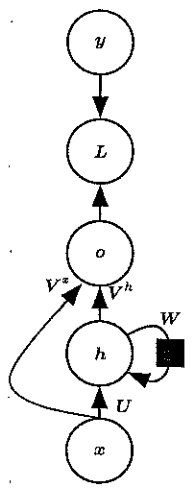
\includegraphics[width=3cm]{Images/io-isomorphic-rnn.jpg}
    \label{fig:io-rnn}
\end{figure}

where $y$ is the target, $L$ the loss function, $o$ the Recurrent Neural Network output, $h$ the hidden state, $x$ the input at time $t$, and the black square represents the time-shift operator $q^{-1}$. $U$, $V^{x}$, $W$ and $V^{h}$ are weight matrices. Suppose to use BPTT with mini-batch equal to 3 for training. Given input sequences composed of 3 items, how many terms should be summed up to compute the gradient of the loss with respect to U?

\newpage
\noindent 13. Suppose to have IO-isomorphic prediction task and a the following Recurrent Neural Network:

\begin{figure}[h]
    \centering
    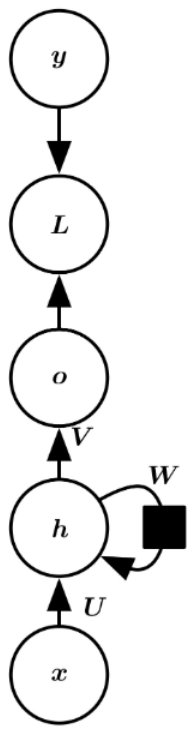
\includegraphics[width=2cm]{Images/io-isomorphic-rnn2.jpg}
    \label{fig:io-rnn2}
\end{figure}

where $y$ is the target, $L$ the loss function, $o$ the Recurrent Neural Network output, $h$ the hidden state, $x$ the input at time $t$, and the black square represents the time-shift operator $q^{-1}$. $U$, $V$ and $W$ are weight matrices. Suppose to use BPTT with mini-batch equal to 1 for training. Given input sequences composed of 4 items, how many terms should be summed up to compute the gradient of the loss with respect to W?


\noindent 14. Suppose to have IO-isomorphic prediction task and a the following Recurrent Neural Network that works only for odd time stamps $t=1, 3, 5, ...$:

\begin{figure}[h]
    \centering
    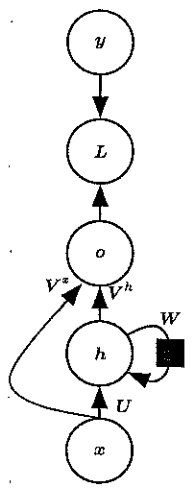
\includegraphics[width=3cm]{Images/io-isomorphic-rnn.jpg}
    \label{fig:io-rnn}
\end{figure}

where $y$ is the target, $L$ the loss function, $o$ the Recurrent Neural Network output, $h$ the hidden state, $x$ the input at time $t$, and the black square represents the time-shift operator $q^{-1}$. $U$, $V^{x}$, $W$ and $V^{h}$ are weight matrices. Suppose to use BPTT with mini-batch equal to 3 for training. Given input sequences composed of 6, 4 and 2 items, how many terms should be summed up to compute the gradient of the loss with respect to W?

\newpage
\noindent 15. Suppose to have IO-isomorphic prediction task and a the following Recurrent Neural Network:

\begin{figure}[h]
    \centering
    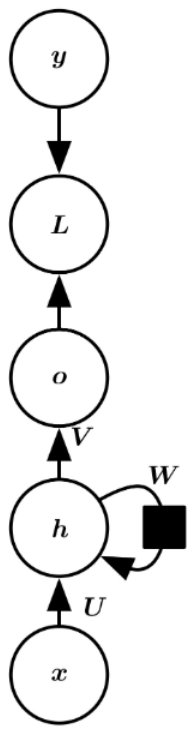
\includegraphics[width=2cm]{Images/io-isomorphic-rnn2.jpg}
    \label{fig:io-rnn2}
\end{figure}

where $y$ is the target, $L$ the loss function, $o$ the Recurrent Neural Network output, $h$ the hidden state, $x$ the input at time $t$, and the black square represents the time-shift operator $q^{-1}$. $U$, $V$ and $W$ are weight matrices. Suppose to use BPTT with mini-batch equal to 1 for training. Given input sequences composed of 4 items, how many terms should be summed up to compute the gradient of the loss with respect to U?


\noindent 16. Suppose to have IO-isomorphic prediction task and a the following Recurrent Neural Network:

\begin{figure}[h]
    \centering
    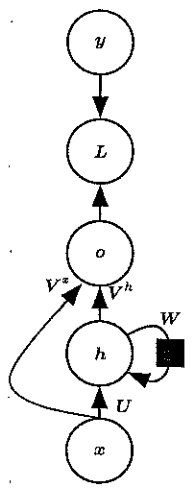
\includegraphics[width=3cm]{Images/io-isomorphic-rnn.jpg}
    \label{fig:io-rnn}
\end{figure}

where $y$ is the target, $L$ the loss function, $o$ the Recurrent Neural Network output, $h$ the hidden state, $x$ the input at time $t$, and the black square represents the time-shift operator $q^{-1}$. $U$, $V^{x}$, $W$ and $V^{h}$ are weight matrices. Suppose to use BPTT with mini-batch equal to 2 for training. Given input sequences composed of 3 items, how many terms should be summed up to compute the gradient of the loss with respect to U?

\newpage
\noindent 17. Suppose to have IO-isomorphic prediction task and a the following Recurrent Neural Network:

\begin{figure}[h]
    \centering
    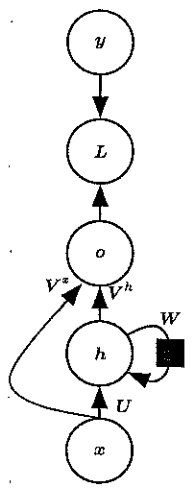
\includegraphics[width=3cm]{Images/io-isomorphic-rnn.jpg}
    \label{fig:io-rnn}
\end{figure}

where $y$ is the target, $L$ the loss function, $o$ the Recurrent Neural Network output, $h$ the hidden state, $x$ the input at time $t$, and the black square represents the time-shift operator $q^{-1}$. $U$, $V^{x}$, $W$ and $V^{h}$ are weight matrices. Suppose to use BPTT with mini-batch equal to 3 for training. Given input sequences composed of 5 items, how many terms should be summed up to compute the gradient of the loss with respect to U?


\noindent 18. Suppose to have IO-isomorphic prediction task and a the following Recurrent Neural Network:

\begin{figure}[h]
    \centering
    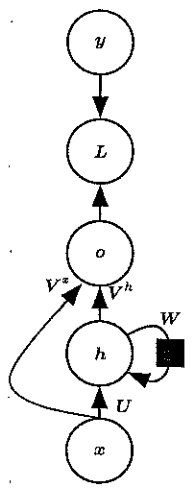
\includegraphics[width=3cm]{Images/io-isomorphic-rnn.jpg}
    \label{fig:io-rnn}
\end{figure}

where $y$ is the target, $L$ the loss function, $o$ the Recurrent Neural Network output, $h$ the hidden state, $x$ the input at time $t$, and the black square represents the time-shift operator $q^{-1}$. $U$, $V^{x}$, $W$ and $V^{h}$ are weight matrices. Suppose to use BPTT with mini-batch equal to 2 for training. Given input sequences composed of 4 items, how many terms should be summed up to compute the gradient of the loss with respect to U?

\newpage
\noindent 19. Suppose to have IO-isomorphic prediction task and a the following Recurrent Neural Network:

\begin{figure}[h]
    \centering
    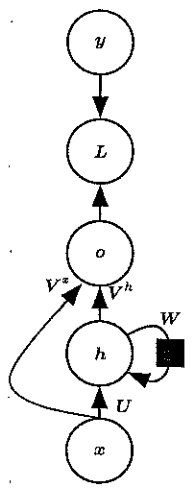
\includegraphics[width=3cm]{Images/io-isomorphic-rnn.jpg}
    \label{fig:io-rnn}
\end{figure}

where $y$ is the target, $L$ the loss function, $o$ the Recurrent Neural Network output, $h$ the hidden state, $x$ the input at time $t$, and the black square represents the time-shift operator $q^{-1}$. $U$, $V^{x}$, $W$ and $V^{h}$ are weight matrices. Suppose to use BPTT with mini-batch equal to 2 for training. Given input sequences composed of 4 items, how many terms should be summed up to compute the gradient of the loss with respect to W?

\noindent 20. Suppose to have IO-isomorphic prediction task and a the following Recurrent Neural Network:

\begin{figure}[h]
    \centering
    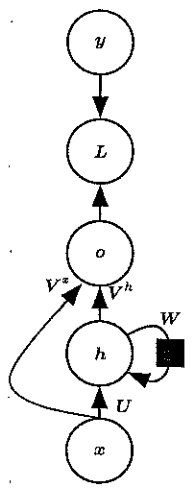
\includegraphics[width=3cm]{Images/io-isomorphic-rnn.jpg}
    \label{fig:io-rnn}
\end{figure}

where $y$ is the target, $L$ the loss function, $o$ the Recurrent Neural Network output, $h$ the hidden state, $x$ the input at time $t$, and the black square represents the time-shift operator $q^{-1}$. $U$, $V^{x}$, $W$ and $V^{h}$ are weight matrices. Suppose to use BPTT with mini-batch equal to 2 for training. Given input sequences composed of 2 and 4 items, how many terms should be summed up to compute the gradient of the loss with respect to U?



\noindent 21. In the context of sequential transductions, give the definition of causality and discuss how this concept is implemented in Recurrent Neural Networks. Are all Recurrent Neural Networks architectures causal?

\newpage
\noindent 22. Give the definition of a sequential transduction, explaining the concept of memory, causality, and recursive state representation. For each different type of sequential transduction describe a network architecture able to implement it.

\noindent 23. Present and motivate the different architectural features that a Recurrent Neural Network can posses.

\noindent 24. Discuss the differences between Backpropagation Through Time and Real-Time Recurrent Learning.

\noindent 25. Introduce the GRU formula and explain it.

\noindent 26. What is a LSTM and explain the role of its components?

\noindent 27. Explain what a Reservoir Computing Network is. What are the main features and properties that such model owns?


\noindent 28. Giving the Recurrent Neural Network defined with the following equations and loss function L:

$$ h^{(0)} = 0  ~~~~ a_{h}^{(t)} = Ux^{(t)} + Wh^{(t-1)} + b  ~~~~ h^{(t)} = ReLU(a_{h}^{(t)}) $$
$$ a_{0}^{(t)} = V h^{(t)} + c ~~~~ o^{(t)} = \sigma \left( a_{0}^{(t)} \right) ~~~~ L = \sum_{t} e^{(t)} = \sum_{t} \left( y^{(t)} - o^{(t)} \right)^{2} $$

\noindent Consider the following learning task involving a single sequence:

input sequence   ~~~~~~ target sequence

$ \begin{pmatrix} 1 \\ -1 \end{pmatrix} \leftarrow  \begin{pmatrix} 1 \\ 1 \end{pmatrix}  ~~~~~~~~~~  \begin{pmatrix} 1 \end{pmatrix} \leftarrow  \begin{pmatrix} -1 \end{pmatrix}  $ 

$ t = 1  ~~~~~~ t = 2  ~~~~~~~~~ t=1 ~~~~ t=2$

\noindent Assume the following values for the parameters:

$ U = \begin{pmatrix} 2 & 0 \\ 2 & 2  \end{pmatrix} $, $ W = \begin{pmatrix} -1 & 1 \\ 0 & 1  \end{pmatrix} $, $ V = \begin{pmatrix} 1 & -1 \end{pmatrix} $, $ b = \begin{pmatrix} 2 \\ 2 \end{pmatrix} $, $c=6$. 

\noindent Compute the gradient $ \frac{\partial o^{(t=2)}}{\partial U} $ using BPTT.

\noindent 29. Giving the Recurrent Neural Network defined with the following equations and loss function L:

$$ h^{(0)} = 0  ~~~~ a_{h}^{(t)} = Ux^{(t)} + Wh^{(t-1)} + b  ~~~~ h^{(t)} = ReLU(a_{h}^{(t)}) $$
$$ a_{0}^{(t)} = V h^{(t)} + c ~~~~ o^{(t)} = \sigma \left( a_{0}^{(t)} \right) ~~~~ L = \sum_{t} e^{(t)} = \sum_{t} \left( y^{(t)} - o^{(t)} \right)^{2} $$

\noindent Consider the following learning task involving a single sequence:

input sequence   ~~~~~~ target sequence

$ \begin{pmatrix} 2 \\ 1 \end{pmatrix} \leftarrow  \begin{pmatrix} 1 \\ -1 \end{pmatrix}  ~~~~~~~~~~  \begin{pmatrix} 1 \end{pmatrix} \leftarrow  \begin{pmatrix} -1 \end{pmatrix}  $ 

$ t = 1  ~~~~~~ t = 2  ~~~~~~~~~ t=1 ~~~~ t=2$

\noindent Assume the following values for the parameters:

$ U = \begin{pmatrix} 1 & 2 \\ 2 & -1  \end{pmatrix} $, $ W = \begin{pmatrix} 2 & 3 \\ 1 & -1  \end{pmatrix} $, $ V = \begin{pmatrix} 1 & -2 \end{pmatrix} $, $ b = \begin{pmatrix} 2 \\ 2 \end{pmatrix} $, $c=6$. 

\noindent Compute the gradient $ \frac{\partial o^{(t=2)}}{\partial W} $ using BPTT.


\section{ GCNN}

1. Explain how a Graph Convolutional Neural Network is different from a Convolutional Neural Network for images.

\noindent 2. What is a Graph Convolutional Neural Network? Explain how it is formulated in the graph spectral domain and in the node domain.

\section{ Autoencoders}

1. The main feature of a denoising autoencoder is:

\begin{enumerate}[label=\roman*]
    \item The use of an architecture with a hidden layer with a number of units that is much lower that the dimension of the input space.
    \item The use of an architecture with a hidden layer of linear units.
    \item The use of data that has been processed to remove noise.
    \item The use of an architecture with a first recurrent layer of sigmoid units to reduce the noise in the input.
    \item The use of input data corrupted by noise.
\end{enumerate}

\noindent 2. The encoding network is:

\begin{enumerate}[label=\roman*]
    \item Any network that maps the input of dimension $n$ into a hidden representation of size $m$ where $n >> m$.
    \item It is the initial part of any autoencoder.
    \item It is the network obtained by unrolling a Recurrent Neural Network on a specific sequence in input.
    \item It is the initial part the Autoencoder for which the size m of the hidden representation is smaller of the dimension n of the input data.
    \item None are correct.
\end{enumerate}

\noindent 3. Define a Sparse Autoencoder. Explain the differences with respect to an Undercomplete Autoencoder.

\noindent 4. Define a contractive Autoencoder. Explain the differences with respect to an undercomplete Autoencoder.

\section{ Probabilistic Models}

1. Given stochastic variables $X_1$, $X_2$, $X_3$, $X_4$ and the fact that:

\begin{itemize}
    \item $X_2$ is conditionally independent from $X_3$ given $X_4$
    \item $X_1$ is conditionally independent from $X_4$ given $X_2$
\end{itemize}

\noindent the joint probability distribution $P(X_1, X_2, X_3, X_4)$ can be factorized as:
\begin{enumerate}[label=\roman*]
    \item $P(X_2)P(X_4 | X_2)P(X_1 | X_2) P(X_3 | X_1, X_2, X_4)$
    \item $P(X_1) P(X_2) P(X_3) P(X_4 | X_3, X_2)$
    \item $P(X_3) P(X_2 | X_1) P(X_3 | X_1) P(X_4 | X_2)$
    \item $P(X_1) P(X_2 | X_1) P(X_3 | X_2) P(X_4 | X_3)$
    \item $P(X_3) P(X_2 | X_1) P(X_3 | X_1) P(X_4 | X_2)$
\end{enumerate}

\newpage

\noindent 2. Given stochastic variables $X_1$, $X_2$, $X_3$, $X_4$ and the fact that:

\begin{itemize}
    \item $X_1$ is conditionally independent from $X_4$ given $X_2$ and $X_3$
    \item $X_1$ is conditionally independent from $X_3$ given $X_2$
\end{itemize}

\noindent the joint probability distribution $P(X_1, X_2, X_3, X_4)$ can be factorized as:
\begin{enumerate}[label=\roman*]
    \item $P(X_1)P(X_2 | X_1)P(X_3 | X_2, X_1) P(X_4 | X_3, X_2, X_1)$
    \item $P(X_1) P(X_2) P(X_3) P(X_4 | X_3, X_2)$
    \item $P(X_1) P(X_2 | X_1) P(X_3 | X_1) P(X_4 | X_2)$
    \item $P(X_1) P(X_2 | X_1) P(X_3 | X_2) P(X_4 | X_1)$
    \item $P(X_1) P(X_2 | X_1) P(X_3 | X_1) P(X_4 | X_1)$
\end{enumerate}

\noindent 3. Given stochastic variables $X_1$, $X_2$, $X_3$, $X_4$, $X_5$ and the fact that:

\begin{itemize}
    \item $X_5$ is conditionally independent from $X_3$ given $X_4$
    \item $X_4$ is conditionally independent from $X_1$ given $X_3$
    \item $X_3$ is conditionally independent from $X_2$ given $X_1$
\end{itemize}

\noindent the joint probability distribution $P(X_1, X_2, X_3, X_4, X_5)$ can be factorized as:
\begin{enumerate}[label=\roman*]
    \item $P(X_1)P(X_4 | X_2, X_1)P(X_2 |X_1) P(X_3 | X_1) P(X_5 | X_4, X_2, X_1)$
    \item $P(X_2 | X_1) P(X_4 | X_3, X_2) P(X_1) P(X_5) P(X_5 | X_4, X_2, X_1)$
    \item $P(X_1) P(X_4 | X_3, X_1) P(X_3 | X_2) P(X_2 | X_1) P(X_5 | X_4, X_3, X_2, X_1)$
    \item $ P(X_5 | X_4, X_3, X_2, X_1) P(X_4| X_3, X_2) P(X_3 | X_2) P(X_2 | X_1) P(X_1)$
    \item None of the above
\end{enumerate}


\noindent 4. Given stochastic variables $X_1$, $X_2$, $X_3$, $X_4$ and the fact that:

\begin{itemize}
    \item $X_4$ is conditionally independent from $X_3$ given $X_2$
    \item $X_3$ is conditionally independent from $X_2$ given $X_1$
\end{itemize}

\noindent the joint probability distribution $P(X_1, X_2, X_3, X_4)$ can be factorized as:
\begin{enumerate}[label=\roman*]
    \item $P(X_1)P(X_4 | X_2, X_1)P(X_2 | X_1) P(X_3 | X_1)$
    \item $P(X_1) P(X_4 | X_3, X_1) P(X_3 | X_2) P(X_2 | X_1)$
    \item $P(X_2 | X_1) P(X_4 | X_3, X_2) P(X_3 | X_1) P(X_1)$
    \item $P(X_4 | X_3, X_2) P(X_3 | X_2) P(X_2 | X_1) P(X_1)$
    \item $P(X_3 | X_1) P(X_2 | X_1) P(X_1) P(X_4 | X_3, X_1)$
\end{enumerate}


\newpage
\noindent 5. Given the following undirected graph or Markov network:

\begin{figure}[h]
    \centering
    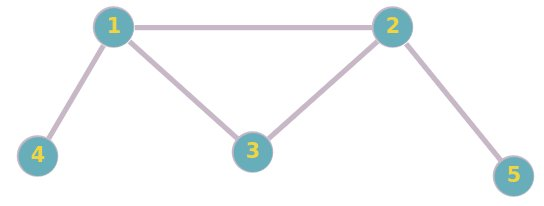
\includegraphics[width=6cm]{Images/undirected-exercise.jpg}
    \label{fig:exercise-markov}
\end{figure}

\noindent Choose the TRUE statement:

\begin{enumerate}[label=\roman*]
    \item $X_4$ and $X_5$ are separated if $X_3$ observed.
    \item $X_4$ and $X_5$ are not separated if $X_2$ observed.
    \item $X_4$ and $X_5$ are separated if $X_1$ observed.
    \item $X_3$ and $X_4$ are not separated if $X_1$ observed.
    \item All are false.
\end{enumerate}

\noindent 6. Given the following undirected graph or Markov network:

\begin{figure}[h]
    \centering
    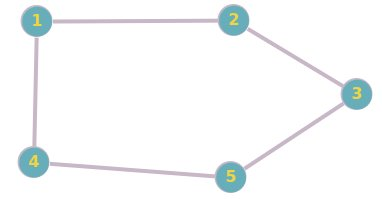
\includegraphics[width=6cm]{Images/undirected-exercise2.jpg}
    \label{fig:exercise-markov}
\end{figure}

\noindent Choose the TRUE statements:

\begin{enumerate}[label=\roman*]
    \item $X_4$ and $X_3$ are separated if $X_5$ observed.
    \item $X_1$ and $X_5$ are not separated if $X_2$ observed.
    \item $X_4$ and $X_5$ are separated if $X_1$ observed.
    \item $X_3$ and $X_4$ are not separated if $X_1$ observed.
    \item All are false.
\end{enumerate}



\noindent 7. Consider the following Bayesian network

\begin{figure}[h]
    \centering
    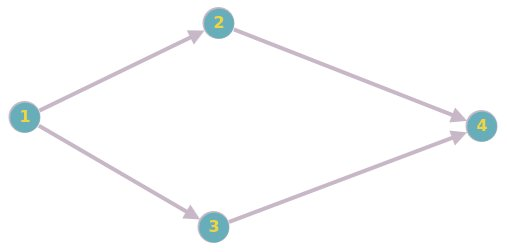
\includegraphics[width=6cm]{Images/directed-exercise.jpg}
    \label{fig:exercise-bayesian}
\end{figure}

\noindent and $|{X_i}| = v$ where $X_i$ can take $v$ values:

\begin{itemize}
    \item $S_1$: $|X_1| = 4$, $|X_2| = 2$, $|X_3| = 3$, $|X_4| = 4$
    \item $S_2$: $|X_1| = 5$, $|X_2| = 3$, $|X_3| = 2$, $|X_4| = 2$
    \item $S_3$: $|X_1| = 3$, $|X_2| = 5$, $|X_3| = 2$, $|X_4| = 3$
    \item $S_4$: $|X_1| = 2$, $|X_2| = 2$, $|X_3| = 5$, $|X_4| = 5$
    \item $S_5$: $|X_1| = 5$, $|X_2| = 5$, $|X_3| = 2$, $|X_4| = 2$
    \item $S_6$: $|X_1| = 5$, $|X_2| = 2$, $|X_3| = 5$, $|X_4| = 2$
\end{itemize}

\noindent The number of necessary parameters for the Bayesian network:

\begin{enumerate}[label=\roman*]
    \item In $S_1$ is less than in $S_2$.
    \item In $S_5$ is more than in $S_6$.
    \item In $S_4$ is less than in $S_3$.
    \item In $S_5$ is more than in $S_4$.
    \item All statements are false.
\end{enumerate}


\noindent 8. Consider the following Bayesian network

\begin{figure}[h]
    \centering
    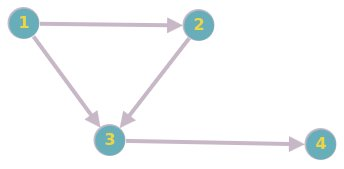
\includegraphics[width=6cm]{Images/directed-exercise2.jpg}
    \label{fig:exercise-bayesian}
\end{figure}

\noindent and $|{X_i}| = v$ where $X_i$ can take $v$ values:

\begin{itemize}
    \item $S_1$: $|X_1| = 4$, $|X_2| = 2$, $|X_3| = 3$, $|X_4| = 4$
    \item $S_2$: $|X_1| = 5$, $|X_2| = 3$, $|X_3| = 2$, $|X_4| = 2$
    \item $S_3$: $|X_1| = 3$, $|X_2| = 5$, $|X_3| = 2$, $|X_4| = 3$
    \item $S_4$: $|X_1| = 2$, $|X_2| = 2$, $|X_3| = 5$, $|X_4| = 5$
    \item $S_5$: $|X_1| = 5$, $|X_2| = 5$, $|X_3| = 2$, $|X_4| = 2$
    \item $S_6$: $|X_1| = 5$, $|X_2| = 2$, $|X_3| = 5$, $|X_4| = 2$
\end{itemize}

\noindent Calculate the number of necessary parameters for each Bayesian network.


\noindent 9. What is the difference between a probabilistic model represented by a directed graph and one represented by an undirected graph? Explain the pros and cons of each representation.

\section{ MonteCarlo Methods and Restricted Boltzmann Machines}

1. Training a Restricted Boltzmann Machine is performed thanks to:

\begin{enumerate}[label=\roman*]
    \item The standard backpropagation algorithm.
    \item Gradient Descent + ancestral sampling.
    \item Gradient Ascent + ancestral sampling.
    \item A multiphase algorithm based only on Gibbs sampling.
    \item Gradient Ascent + Gibbs sampling.
\end{enumerate}


\noindent 2. Explain in detail what is the role of MonteCarlo chains in the training of a stochastic Neural Networks. Give an example of a Neural Network model where MonteCarlo chains are used.

\noindent 3. What is a MonteCarlo chain? Explain why it is an important concept. Describe an algorithm for sampling from a MonteCarlo chain.

\noindent 4. Present in detail the stochastic maximum likelihood / persistent contrastive divergence algorithm using gradient ascent for Restrictive Boltzmann Machines.

\newpage
\noindent 5. In the context of learning in Restrictive Boltzmann Machines, write all the steps to prove the following result:

$$ \frac{\partial \log \left( p(x \vert \theta) \right)}{ c_z } = \sum_{i=1}^{m} \sigma \left(  c_z + v^{T} W_{:, z} \right) - \sum_{v} p(v) \sigma \left( c_z + v^{T} W_{:, z} \right)   $$


\noindent 6. In the context of Restricted Boltzmann networks, write all the steps to prove the following results:

$$ P(v \vert h) = \prod_{i=1}^{n_v} \sigma \left( (2v -1) \odot (b + Wh) \right)_i     $$


\section{ Variational Autoencoders \& Generative Adversarial Networks}

\noindent 1. What is a Differentiable Generator Network? Why it is useful? Give a simple example of a Differentiable Generator Network.

\noindent 2. Define a Variational Autoencoder. Explain how it is used for and how it can be trained.

\noindent 3. Explain the meaning of the acronym ELBO, giving all technical details related to it. In addition, explain why ELBO is important.


\noindent 4. Define a Generative Adversarial Network. Explain why it is useful and how it can be trained. 


\noindent 5. Introduce the objective function used in Generative Adversarial Networks and explain it.

\noindent 6. Why Generative Adversarial Networks are useful? Describe and explain the mathematics of its training algorithm.

